\documentclass[conference]{IEEEtran}
\IEEEoverridecommandlockouts
% The preceding line is only needed to identify funding in the first footnote. If that is unneeded, please comment it out.
\usepackage{cite}
\usepackage{amsmath,amssymb,amsfonts}
\usepackage{tabularx,booktabs}
% defined centered version of "X" column type:
\newcolumntype{C}{>{\centering\arraybackslash}X} 
\setlength{\extrarowheight}{1pt} % for a bit more open "look
\DeclareUnicodeCharacter{2009}{\,} 
\usepackage{graphicx}
\usepackage{caption}
\usepackage{subcaption}
\usepackage{hyperref}
\usepackage{textcomp}
\usepackage{xcolor}
\usepackage{multirow}
\usepackage{mathtools, cuted}
\usepackage{algorithm}
\usepackage{algpseudocode}
\usepackage{graphicx}
\def\BibTeX{{\rm B\kern-.05em{\sc i\kern-.025em b}\kern-.08em
    T\kern-.1667em\lower.7ex\hbox{E}\kern-.125emX}}

\makeatletter
\newcommand{\linebreakand}{%
  \end{@IEEEauthorhalign}
  \hfill\mbox{}\par
  \mbox{}\hfill\begin{@IEEEauthorhalign}
}
\makeatother

\begin{document}%
\title{Attractor inspired Deep Learning for Modelling Chaotic Systems}
%
%\titlerunning{Abbreviated paper title}
% If the paper title is too long for the running head, you can set
% an abbreviated paper title here
%
\author{\IEEEauthorblockN{1\textsuperscript{st} Anurag Dutta}
\IEEEauthorblockA{\textit{Department of Computer Science} \\
\textit{Government College of Engineering \& Textile Technology}\\
Serampore, Calcutta, India \\
anuragdutta.research@gmail.com}
}

%
\maketitle              % typeset the header of the contribution
%
\begin{abstract}
Due to its unrivalled performance in numerous areas, including computer vision, processing natural languages, recommendation engines, and also most notably in modelling simulation issues and forecasting complex system dynamics, deep learning has gained greater prominence. Yet, because deep learning models need huge data to be trained, which is frequently not available, modelling and predicting the behaviour of stochastic processes constitute unresolved research questions. By applying the fundamental laws governing non-linear system and using deeper knowledge gleaned from simulation, these deep learning can be performed. In this study, appealing frameworks constructed using deep neural networks, known as Attractor inspired Deep Learning (AiDL) models, are proposed. These models take into account severe occurrences and their evolution. By concurrently learning upon actual and simultaneously from the complexities and associated mathematical models, our hypothesized AiDL may comprehend the swirls underlying Chaotic Attractors. This understanding is applied to anticipate and simulate turbulent real-world phenomena with aberrant behaviour. \\
\end{abstract}

\begin{IEEEkeywords}
Chaotic Systems, Attractor, Deep Learning, Artificial Intelligence, Butterfly Effect
\end{IEEEkeywords}
%
%
%
\section{Introduction}\label{sec1}
A variety of prediction approaches, features extraction methods, and large-scale computations have all advanced as a result of millennia attempts to understand and predict the evolution of dynamic systems [1, 2, 3]. Predetermined dynamical systems known as chaotic systems [4] display stochastic nature [5] across time as well as occasionally defy prediction. To characterize the temporal as well as spatial relationships [6] of these entities, physical principles may be employed as models. Several complex systems developed to comprehend naturally occurring phenomena, their erratic behaviour, and the manner in which a modification in the beginning circumstances of actual situations could result in a random change in the solution. Throughout the past several decades, computation methods and fundamental rules have been used to further the objectives of comprehending and forecasting non-linear system. Given advances in processing power, computational advancements, and the abundance of data, we have seen a confluence of such techniques towards contemporary information-driven techniques in recent decades. Approaches to machine learning centred around physics, dynamical understanding using deep neural networks [7, 8], including portrayal learning for studying continual system dynamics and biochemical factors [9, 10, 11] are all key beneficiaries of this integration.\\

A deterministic non-linear system's butterfly effect [12-16] is a delicate dependency on beginning circumstances where a slight modification during one phase can have a significant impact on a subsequent phase. Henri Poincaré [17], a French mathematician and scientist, was the initial individual to recognise that meteorology can be influenced by little factors which could have big impacts. Norbert Wiener, renowned American scientist and theologian, also made a contribution to this idea. With his research, Lorenz gave the idea of the Earth's atmosphere and oceans unpredictability a quantifiable foundation and connected the idea to the characteristics of sizeable categories of chaotic environments that are experiencing dynamic behaviour and predictable chaos. Figure 1 depicts a Graphical Plot of the Lorenz's Strange Attractor [18, 19], which ascertains itself with the Butterfly Effect. Equations \ref{eq1}, \ref{eq2}, and \ref{eq3} represents the dynamics of the Lorenz Attractors. 
\begin{equation}\label{eq1}
\frac{dx}{dt}=\sigma\left(y-x\right)
\end{equation}
\begin{equation}\label{eq2}
\frac{dy}{dt}=x\left(\rho-z\right)-y
\end{equation}
\begin{equation}\label{eq3}
\frac{dz}{dt}=xy-\beta z
\end{equation}
\begin{figure}
\centerline{\includegraphics[width = \linewidth]{1.png}}
\caption{Lorenz's weird vortex plotted for constants of $\rho=28$, $\sigma=10$, and $\beta=\frac{8}{3}$. The Butterfly Effect, also known as hypersensitive dependency on initial values, is a dynamic nonlinear feature that causes the sequential positions becoming indefinitely split apart from one another commencing with any of several relatively comparable potential initial state upon that attractor.}
\end{figure}
Freak occurrences that are extremely susceptible to perturbations, including natural disasters [20] and meteorological patterns [21], are frequently referred to as chaotic systems. whereas the climate can be expected immediately, in the immediate future, but some unforeseen events make long-term forecasting difficult. Dynamical systems, a non-linear expression of the feature expressing the spatio-temporal interdependence seen between system's components, are being used to characterize non-linear system. When distortion or disturbance is prevalent, particularly is consistently the situation in chaotic systems, physics-driven techniques are able to anticipate non-linear system in the shorter term but are unable to foresee important considerations. However, certain non-linearities cannot be modelled using direct simulation analysis because of the intricate nature of the kinematics, which reduces the accuracy of the forecast and raises the degree of ambiguity in the interpretation of the physical methods. Yet, enormous volumes of data are required for training deep neural network algorithms in information-driven methodologies to predict and anticipate non-linear system. Whenever the system's behaviour is unpredictable, things are hard to draw conclusions and frequently fall short of simulating long-term dependence. Several studies concentrated on modelling non-linear system employing deep learning by incorporating prior knowledge, particularly when testing data was scarce. A promising area of research may be capable of solving the enduring problems of modelling non-linear system by integrating spatial quantities into simulations of real-world occurrences. With the application of non-linear equations, physics-informed machine learning (PIML) [22], a novel category of approach to machine learning, incorporates past scientific expertise into data-driven computations. When a substantial chunk of time series is needed to provide precise and trustworthy predictions of chaotic systems involving severe occurrences, this method is well suited. It adds physiological expertise into information-driven machine learning algorithms so that it may grasp the complex and comprehensive occurrences rather than solely relying on the information. Physics-informed neural networks (PINN) [23] were presented as a portion of the available in contemporary magnum opus. With a smoothing filter in the error function, PINN is able to produce a precise outcome to the underlying partial derivative equations (PDE) by supplying a number of cluster centroids, the start, and material parameters. When the PDE's indices, beginning or border circumstances are reconstructed and the controlling PDE's workaround is only partially known, PINN may additionally be employed to tackle inverse issues. The circulation inside an expresso cup was one of several implementations for PINN, modelling 3D temperature measurements utilizing known laws of physics in a densely integrated network infrastructure. As a spatio-temporal estimation problem, lake warmth is modelled using physics-guided neural network models (PGNN) [24], a different framework that is comparable. LSTM networks construct the simulation using the fluctuations of temperature at the sea surface. More specifically, the principles and concepts integrate the kinetics by firmly encoding these on a computer granularity inside a PGNN framework for a limited data regime, which enforces the uniformity of densities with detail. \\

The aforementioned approaches, nonetheless, fall short in regard to simulating non-linear system. A PDE's resolution guiding the system's internal processes is modelled and simulated by PINN, which is limited to using to mimic data. Moreover, coordination sites, boundaries, and beginning circumstances are inputs needed for PINN. As a result, some models (like PINN) are only applicable to synthetic information and can't be immediately applied to chaotic model transformation issues in the actual world. \\

We intend to develop a fundamentally coherent and universally applicable deep learning framework for modelling nonlinear system that integrates seamlessly actual statistics and modeled information directly from the kinetics and their mathematical models, prompted by the limitations of the aforementioned methods. In this article, we would focus on proposition of a family of Attractor Inspired Deep Learning Models. For apt disposition of the paradigm, we would make us of some extreme events. The mechanics of catastrophic weather control the cycles of the El Niño surface temperature of the sea, San Juan Dengue virus transmission, and Bjørnøya daily downpour. Section \ref{sec2} discusses about Attractors and their Dynamics. In Section \ref{sec3}, the AiDL proposition is laid. 
\section{Attractors}\label{sec2}
An attractor [25-28] is a group of states that a consensus mechanism to advance towards in the subject of non-linear dynamics mathematics, regardless of the system's initial and boundary conditions. System characteristics that are sufficiently near to the vortex parameters stay there still when they are marginally perturbed. In general, one or maybe more differentiated equations can characterise a chaotic system. A particular non-linear system's behaviour over every given short time frame is described by its characteristics. It is frequently crucial to incorporate the equations in order to predict the behaviour of the system over a longer time period. This can be done analytically or iteratively, frequently with the use of computing. In the material realm, chaotic systems typically develop from viscous dissipation ones because without a propelling source, locomotion would stop. Initial transient response are killed out and the mechanism settles into its regular behaviour as the absorption and the guiding force seek to balance one another. The attractor, which is sometimes referred to as the attractive portion or the attractee, is the component of the chaotic system's dimensional space that corresponds to the appropriate behaviour. The attractor notion is analogous to limit sets as well as invariant sets. A collection that conforms to its own characteristics as the result of kinetics is said to be immutable. Deterministic sets may be present in attractors. A limit set is a collection of elements namely that, as time nears infinity, a baseline state occurs that wind up unreasonably near to the limit imposed. Limit sets are exogenous variables, however not every limit set is an attractor. Some system points may advance to a limit set, yet if other system elements are agitated marginally off the limit set, they may get pushed off and never come back to the limit set's proximity. AiDL, as mentioned previously, is a family of Deep Learning Paradigms. Sticking to that proposition, we define 2 members of the family as an illustration of the genus. We make us of Rössler Attractor [29], and Rabinovich Fabrikant Attractor [30]. Let us each of them. 
\subsection{Rössler Attractor}\label{sec2a}
The Rössler attractor serves as the attractor for such Rössler systems, a set of trio quasi conventional differential equations which describe a consistent dynamical system exhibiting chaotic dynamics due to the attractor's fractal characteristics. The fundamental characteristics of the Rössler process requiring non-linear techniques like Poincaré maps \& bifurcation charts, while some system-specific characteristics can be inferred using linear techniques like eigenvectors. The Rössler attractor were designed to act in the same way to the Lorenz vortex while also being simpler to qualitatively examine, according to the classic Rössler study. At an unsteady reference value, an orbit inside the attractor spirals outward approaching the \textit{x,y} plane. Once the graph has spiralled much further, a secondary new equilibrium influences it, enabling the \textit{z}-dimension to ascend and contort. Even though each parameter oscillates within one predetermined value band, this becomes clear in the temporal domain that the fluctuations are disordered. This attractor resembles the Lorenz attractor in some ways, although it is less complicated with just one manifold. Equations \ref{eq4}, \ref{eq5}, and \ref{eq6} represents the dynamics of the Rössler Attractors. 
\begin{equation}\label{eq4}
\frac{dx}{dt}=-y-z
\end{equation}
\begin{equation}\label{eq5}
\frac{dy}{dt}=x+ay
\end{equation}
\begin{equation}\label{eq6}
\frac{dz}{dt}=b+z(x-c)
\end{equation}
Setting $z=0$ leads to some mathematical elegance of the Attractor. Equations \ref{eq7}, and \ref{eq8} represents the dynamics of the Rössler Attractors, in \textit{x-y} plane. Figure 2 depicts a pictorial representation of the Rössler Attractor in the \textit{x-y} plane.
\begin{equation}\label{eq7}
\frac{dx}{dt}=-y
\end{equation}
\begin{equation}\label{eq8}
\frac{dy}{dt}=x+ay
\end{equation}
\begin{figure}
\centerline{\includegraphics[width = \linewidth]{2.png}}
\caption{Rössler's weird vortex plotted for constants of $a=0.2$. It closely resembles a stereogram}
\end{figure}
\subsection{Rabinovich Fabrikant Attractor}
The Rabinovich-Fabrikant equations are a collection of trio chained normal differential equations that, depending on the model parameters, behave chaotically. Equation \ref{eq9}, \ref{eq10}, and \ref{eq11} represents the dynamics of the Rabinovich Fabrikant Attractor. 
\begin{equation}\label{eq9}
\frac{dx}{dt}=y(z-1+x^2)+\gamma x
\end{equation}
\begin{equation}\label{eq10}
\frac{dy}{dt}=x\left(3x+1-x^2\right)+\gamma y
\end{equation}
\begin{equation}\label{eq11}
\frac{dz}{dt}=-2z\left(\alpha+xy\right)
\end{equation}
Figure 3 depicts a pictorial representation of the Rabinovich Fabrikant Attractor. 
\begin{figure}
\centerline{\includegraphics[width = \linewidth]{3.png}}
\caption{Rabinovich Fabrikant's weird vortex plotted for constants of $\alpha=0.05, \gamma=0.1$. It closely resembles a Gramophone}
\end{figure}
\section{Attractor inspired Deep Learning (AiDL)}\label{sec3}
We propose two species of this genus, one following the Rössler Attractor and Rabinovich Fabrikant Attractor. We take into account a known parameter Attractor system with exogenous harmonic perturbations from their dynamical equations. We create our artificial dataset  employing the Runge-Kutta method [31, 32] to simulate pieces of information from the equations of chaotic differentials. Using the modelled time - series data [33], we build a Recurrent neural network [34] simultaneously applying the physiological law to the structure as a regularisation term. The network picks up intricate patterns from distribution channels of the expected values and historical significance. The temporal component is regarded as an input and the resolution to the non-linear equations as an outcome in the traditional PINN paradigm. Differentiating the richly textured feed - forward neural network [35] and calculating the temporal dependencies using auto-differentiation constitute the process of determining the control parameter. It is challenging to estimate the time derivatives because time - series data are discrete occurrences and do not have a strong mathematical model regulating the covariates in time. We generate discrete components of the time - series data to circumvent this problem. Here, we computed $\frac{dx}{dt}$ as 
\begin{equation}\label{eq12}
\frac{dx}{dt}=\frac{x\left(t+\delta t\right)-x\left(t\right)}{\delta t}
\end{equation}
Time is represented as a chrono in sequential manner for real - time system series information. So, in our study, we select $\delta t=7$, subjective the number of days in a week. Because the transfer function employed in MLP is differentiable, the conventional PINN paradigm backpropagates the temporal implications to modify the network loss. The network predicts the value of $x(t)$, $\frac{dx}{dt}$, and $\frac{d^2x}{dt^2}$. For, Rössler Attractor Inspired Deep Learning, the Loss Function would be, 
\begin{equation}\label{eq13}
\mathfrak{L}_{physical}=RMSE\left(\mathfrak{Y}_{predicted},\ \mathfrak{Y}_{real}\right)\ 
\end{equation}
where, 
\begin{equation*}
\mathfrak{Y}_{predicted}=\left(\frac{d^2y_{pred}}{dt^2}+y_{pred}-a\frac{dy_{pred}}{dt}\right)
\end{equation*}
\begin{equation*}
\mathfrak{Y}_{real}=\left(\frac{d^2y_{real}}{dt^2}+y_{real}-a\frac{dy_{real}}{dt}\right)
\end{equation*}
and RMSE stands for Root mean Squared Error. \\

For, Rabinovich Fabrikant Attractor Inspired Deep Learning, the Loss Function would be, 
\begin{strip}
\begin{equation}\label{eq14}
\mathfrak{L}_{physical}=RMSE\left(\mathfrak{Y}_{predicted},\ \mathfrak{Y}_{real}\right)\ 
\end{equation}
where, 
\begin{equation*}
\mathfrak{Y}_{predicted}=\frac{d^2y_{pred}}{dt^2}-\left(\frac{dy_{pred}}{dt}\right)\left(2yy_{pred}+\gamma\right)+\left({y_{pred}}^5-3{y_{pred}}^4-2{y_{pred}}^3-{y_{pred}}^2\left(\gamma y-3\right)+y_{pred}+\gamma y\right)
\end{equation*}
\begin{equation*}
\mathfrak{Y}_{real}=\frac{d^2y_{real}}{dt^2}-\left(\frac{dy_{real}}{dt}\right)\left(2yy_{real}+\gamma\right)+\left({y_{real}}^5-3{y_{real}}^4-2{y_{real}}^3-{y_{real}}^2\left(\gamma y-3\right)+y_{real}+\gamma y\right)
\end{equation*}
\end{strip}
RMSE stands for Root mean Squared Error and
\begin{equation}\label{eq15}
\left(\frac{\frac{dx}{dt}-\gamma x}{x^2-1}\right)=y
\end{equation}
Here, using the AiDL, we will compute $x\left(t+1\right)$, $\frac{d}{dt}\left(x\left(t+1\right)\right)$, and $\frac{d^2}{dt^2}\left(x\left(t+1\right)\right)$, that are the essentials for the next stage. Computaion of these, may result in an additional Loss, generically mentioned as $\mathfrak{L}_{data}$.
\begin{equation}\label{eq16}
\mathfrak{L}_{data}=RMSE\left(\mathfrak{X}_{predicted},\ \mathfrak{X}_{real}\right)
\end{equation}
where,
\begin{equation*}
\mathfrak{X}_{predicted}=x_{pred}\left(t+1\right),\left(x_{pred}\left(t+1\right)\right)^\prime,\left(x_{pred}\left(t+1\right)\right)^{\prime\prime}
\end{equation*}
\begin{equation*}
\mathfrak{X}_{real}=x_{real}\left(t+1\right),\left(x_{real}\left(t+1\right)\right)^\prime,\left(x_{real}\left(t+1\right)\right)^{\prime\prime}
\end{equation*}
Algorithm \ref{alg1} presents the PseudoCode for AiDL. 
\begin{algorithm}
\caption{Attractor inspired Deep Learning (AiDL)}\label{alg1}
\begin{algorithmic}[1]
\Require $\left\{x\left(t-i\right)\right\}_{i=1}^k$, $\left\{\frac{d}{dt}x\left(t-i\right)\right\}_{i=1}^k$, and $\left\{\frac{d^2}{dt^2}x\left(t-i\right)\right\}_{i=1}^k$
\Ensure $x\left(t+1\right)$, $\frac{d}{dt}\left(x\left(t+1\right)\right)$, and $\frac{d^2}{dt^2}\left(x\left(t+1\right)\right)$
      \Function{Attractor inspired Deep Learning}{}
		\State Initialize the Weights ($W_i$) and Biases ($B_i$)
                \If{\textit{Pre-training}}
                		\For{$epoch=1$ to $max\_epoch$}
                			\If{\textit{Termination Condition}}
                				\State break
                			\EndIf
                		\State Get $x\left(t+1\right)$, $\frac{d}{dt}\left(x\left(t+1\right)\right)$, $\frac{d^2}{dt^2}\left(x\left(t+1\right)\right)$
                		\State Compute $\mathfrak{L}_{data}=RMSE\left(\mathfrak{X}_{predicted},\ \mathfrak{X}_{real}\right)$
                		\State Compute $\mathfrak{L}_{phy}=RMSE\left(\mathfrak{Y}_{predicted},\ \mathfrak{Y}_{real}\right)$
                		\State Back propagate as $\mathfrak{L}=\mathfrak{L}_{data}+\mathcal{C}_1\times\mathfrak{L}_{physical}$ \Comment{$\mathcal{C}_1$ is the Hyper parameter}
                		\State Save the Weights ($W_i$) and Biases ($B_i$)
                		\EndFor
                \Else
                		\For{$epoch=1$ to $max\_epoch$}
                			\If{\textit{Termination Condition}}
                				\State break
                			\EndIf
                		\State Load the Weights ($W_i$) and Biases ($B_i$)
                		\State Get $x\left(t+1\right)$, $\frac{d}{dt}\left(x\left(t+1\right)\right)$, $\frac{d^2}{dt^2}\left(x\left(t+1\right)\right)$
                		\State Compute $\mathfrak{L}_{data}=RMSE\left(\mathfrak{X}_{predicted},\ \mathfrak{X}_{real}\right)$
                		\State Compute $\mathfrak{L}_{phy}=RMSE\left(\mathfrak{Y}_{predicted},\ \mathfrak{Y}_{real}\right)$
                		\State Back propagate as $\mathfrak{L}=\mathfrak{L}_{data}+\mathcal{C}_2\times\mathfrak{L}_{physical}$ \Comment{$\mathcal{C}_2$ is the Hyper parameter}
                		\EndFor
                \EndIf
      \EndFunction
\end{algorithmic}
\end{algorithm}
\section{Results}\label{sec4}
To validate the AiDL model, we would implement the primitive specie of the genus. We would implement Rössler Attractor inspired Deep Learning Model. We would apply the Model on 3 benchmark Datasets - El Niño surface temperature of the sea, San Juan Dengue virus transmission, and Bjørnøya daily downpour. We have compared the efficiency of the model with prevalent techniques like, Long Short Term Memory. We took into account three widely used measures while judging our models. The forecasting model performs better the smaller their value is. In this study, we made use of the following metrics
\begin{enumerate}
\item Physical Inconsistency
\item Mean Absolute Error
\item Root Mean Squared Error
\end{enumerate}
Sea surface temperature (SST) variations throughout the Pacific occur on a regular basis and are referred to as the El Niño dataframe or ENSO. From January 3, 1990 to April 21, 2021, the El Niño file comprises 1634 weekly recordings of Sea surface temperature in El Niño zone 1 over the Pacific. A univariate time-series information collection called the San Juan dataset shows how dengue infection cases have fluctuated throughout the years. Freak occurrences are exhibited by this illness as a result of the transmission's unpredictability. An influenza pandemic spread by mosquitoes is dengue fever. 1197 observations total from week 17 in 1990 until week 16 in 2013 are included in the dataset. We just take into account the unitary time series with instances reported throughout this time frame. This data set on catastrophic weather was compiled from observations of precipitation in the Bjørnøya region made by the Norwegian Meteorological Service Center. From June 16, 1980, to June 16, 2022, there were 15320 daily samples included in the analysis. 
The observed results are summarized below in Table \ref{tab1} and graphically compared in Figure 4. 
\begin{figure*}[ht]
\centering
\centerline{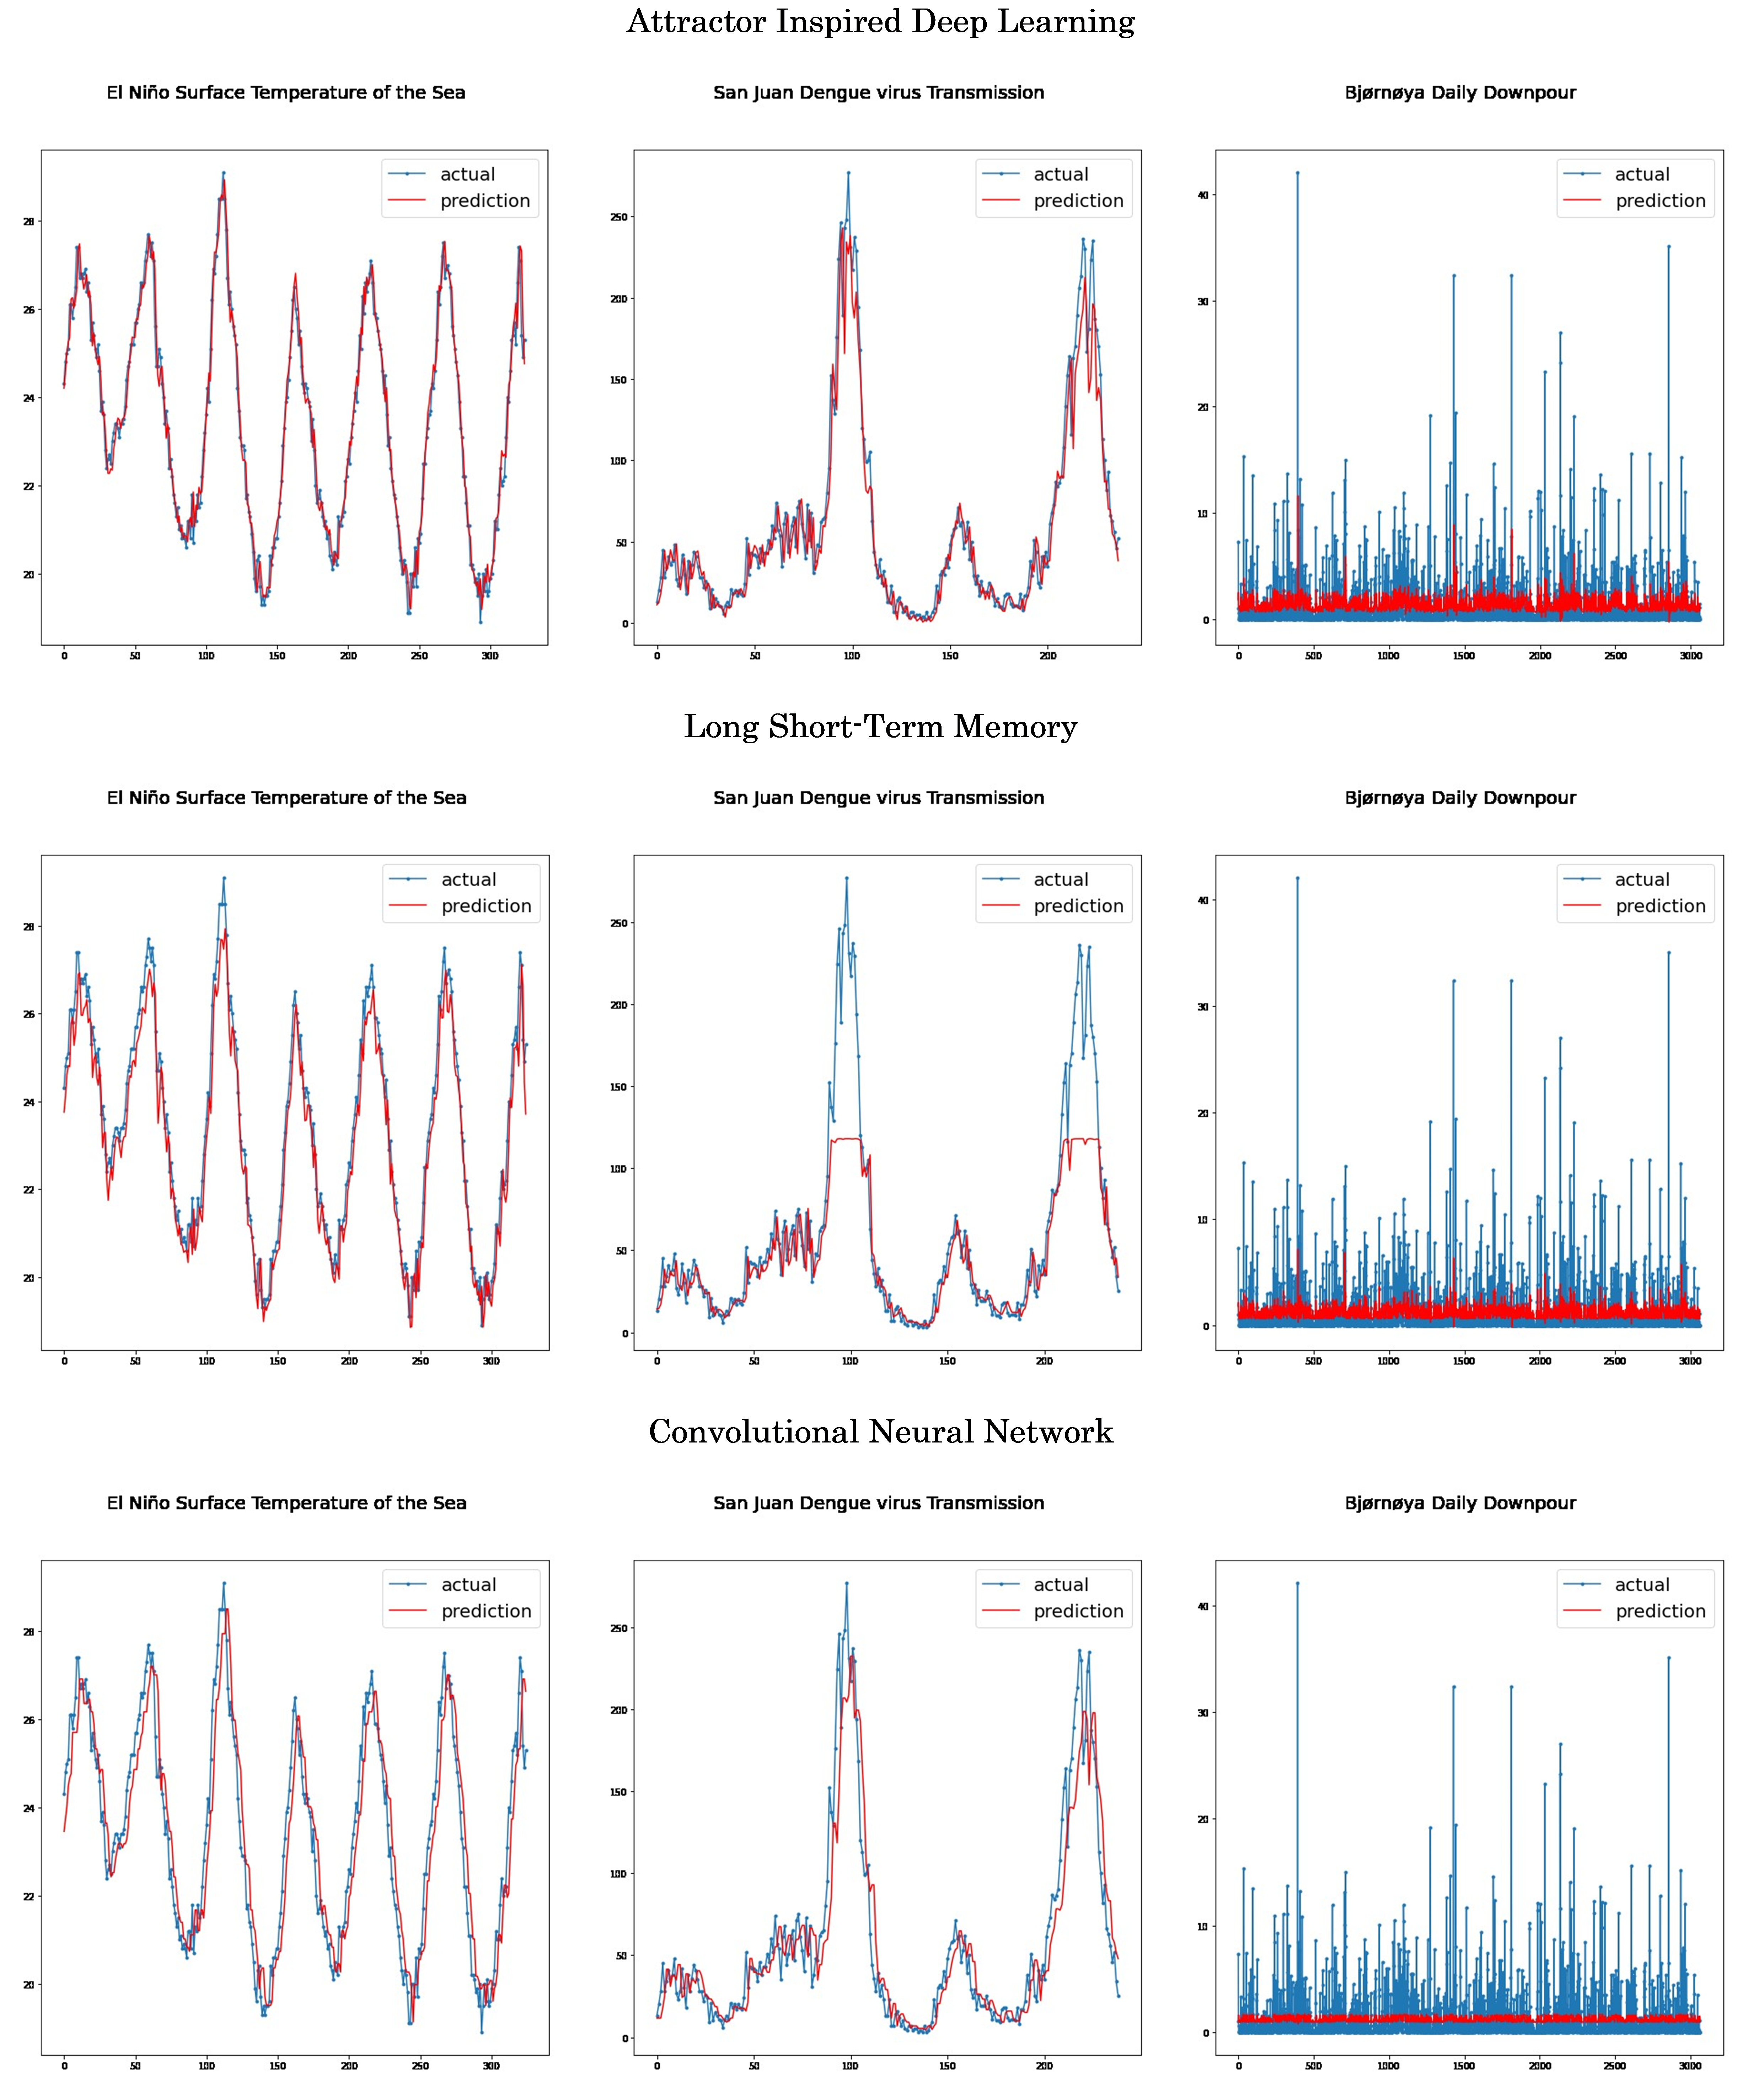
\includegraphics[width = \linewidth]{13.png}}
\caption{Comparative Analysis of the Rössler Attractor inspired Deep Learning Model with Long Short Term Memory Model, and Convolutional Neural Network. }
\end{figure*}
\begin{table*}[htbp]
  \centering
\begin{tabular}{ |p{3cm}||p{3cm}|p{3cm}|p{3cm}|  }
 \hline
 \multicolumn{4}{|c|}{Comparative Analysis between the Algorithms} \\
 \hline
 \textbf{Algorithm Employed}& \textbf{Bjørnøya Daily Downpour} &\textbf{San Juan Dengue virus Transmission}&\textbf{El Niño Surface Temperature of the Sea}\\
 \hline
     & \textbf{Test RMSE: 2.574 }   &\textbf{Test RMSE: 17.185}&   \textbf{Test RMSE: 0.428}\\
 Rössler AiDL&   Test MAE: 1.421  & Test MAE: 11.817   &\textbf{Test MAE: 0.333}\\
  &\textbf{Test PHYS: 3.364} & \textbf{Test PHYS: 28.317}&  \textbf{Test PHYS: 0.822}\\
 \hline
     & Test RMSE: 2.576    &Test RMSE: 34.460&   Test RMSE: 0.614\\
 LSTM&   \textbf{Test MAE: 1.177}  & Test MAE: 4.258   &Test MAE: 0.701\\
  &Test PHYS: N/A & Test PHYS: N/A&  Test PHYS: N/A\\
 \hline
     & Test RMSE: 2.601    &Test RMSE: 23.374&   Test RMSE: 0.858\\
 CNN&   Test MAE: 1.205  & \textbf{Test MAE: 3.892}   &Test MAE: 0.845\\
  &Test PHYS: N/A & Test PHYS: N/A&  Test PHYS: N/A\\
 \hline
\end{tabular}
  \caption{Comparative Analysis of the Rössler Attractor inspired Deep Learning Model with Long Short Term Memory Model, and Convolutional Neural Network on the basis of the 3 errors mentioned in Section \ref{sec4}}
  \label{tab1}
\end{table*}
\section{Conclusion}\label{sec5}
In this article, we suggested an experience and understanding deep learning system that forecasts extreme events by integrating spatial quantities with previously acquired transferrable information from real as well as synthetic data.
The suggested model employs a blended instructional strategies, drawing some of its knowledge from the time - series data, their mechanics, and basic training. Our approach is based on the idea that non-linearities can be described using an oscillator since they produce severe occurrences. This presumption is significantly supported by the fact that our network outperforms all other forecasting techniques taken into account in the analysis. The proposed AiDL methodology with multi-step prediction for future employment is intriguing to think about. The future application of this study's approach to additional pertinent forecasting issues can also be considered. The Codes and the Data have been made available at \href{https://github.com/Anurag-Dutta/AiDL}{https://github.com/Anurag-Dutta/AiDL}. 
\begin{thebibliography}{00}
\bibitem{b1} P. Melby, N. Weber, and A. Hübler, “Dynamics of self-adjusting systems with noise,” \textit{Chaos: An Interdisciplinary Journal of Nonlinear Science}, vol. 15, no. 3, p. 033902, Sep. 2005, doi: https://doi.org/10.1063/1.1953147.
\bibitem{b2} V. Gintautas, G. Foster, and A. W. Hübler, “Resonant Forcing of Chaotic Dynamics,” \textit{Journal of Statistical Physics}, vol. 130, no. 3, pp. 617–629, Oct. 2007, doi: https://doi.org/10.1007/s10955-007-9444-4.
\bibitem{b3} V. Haimo, “Finite time differential equations,” \textit{1985 24th IEEE Conference on Decision and Control}, Dec. 1985, doi: https://doi.org/10.1109/cdc.1985.268832.
\bibitem{b4} C. Werndl, “What Are the New Implications of Chaos for Unpredictability?,” \textit{The British Journal for the Philosophy of Science}, vol. 60, no. 1, pp. 195–220, Mar. 2009, doi: https://doi.org/10.1093/bjps/axn053.
\bibitem{b5} J. L. Doob, “Stochastic Processes and Statistics,” \textit{Proceedings of the National Academy of Sciences}, vol. 20, no. 6, pp. 376–379, Jun. 1934, doi: https://doi.org/10.1073/pnas.20.6.376.
\bibitem{b6} T. Dong, “A COMMENT ON RCC: FROM RCC TO RCC++,” \textit{Journal of Philosophical Logic}, vol. 37, no. 4, pp. 319–352, Jan. 2008, doi: https://doi.org/10.1007/s10992-007-9074-y.
\bibitem{b7} H. Schulz and S. Behnke, “Deep Learning,” \textit{KI - Künstliche Intelligenz}, vol. 26, no. 4, pp. 357–363, May 2012, doi: https://doi.org/10.1007/s13218-012-0198-z.
\bibitem{b8} Y. LeCun, Y. Bengio, and G. Hinton, “Deep Learning,” \textit{Nature}, vol. 521, no. 7553, pp. 436–444, May 2015, doi: https://doi.org/10.1038/nature14539.
\bibitem{b9} B. Srinivasan, “A guide to enzyme kinetics in early drug discovery,” \textit{The FEBS Journal}, Mar. 2022, doi: https://doi.org/10.1111/febs.16404.
\bibitem{b10} N. J. Cobb and W. K. Surewicz, “Prion Diseases and Their Biochemical Mechanisms†,” \textit{Biochemistry}, vol. 48, no. 12, pp. 2574–2585, Mar. 2009, doi: https://doi.org/10.1021/bi900108v.
\bibitem{b11} B. Srinivasan, “A guide to the Michaelis–Menten equation: steady state and beyond,” \textit{The FEBS Journal}, Jul. 2021, doi: https://doi.org/10.1111/febs.16124.
\bibitem{b12} B.-W. Shen et al., “Is Weather Chaotic?: Coexistence of Chaos and Order within a Generalized Lorenz Model,” \textit{Bulletin of the American Meteorological Society}, vol. 102, no. 1, pp. E148–E158, Jan. 2021, doi: https://doi.org/10.1175/BAMS-D-19-0165.1.
‌\bibitem{b13} A. E. Motter and D. K. Campbell, “Chaos at fifty,” \textit{Physics Today}, vol. 66, no. 5, pp. 27–33, May 2013, doi: https://doi.org/10.1063/pt.3.1977.
‌‌\bibitem{b14} P. H. Richter and H.-J. . Scholz, “Chaos in Classical Mechanics: The Double Pendulum,” \textit{Stochastic Phenomena and Chaotic Behaviour in Complex Systems}, pp. 86–97, 1984, doi: https://doi.org/10.1007/978-3-642-69591-9\_9.
‌‌\bibitem{b15} R. A. Anthes, “Predictability and Predictions,” \textit{Atmosphere}, vol. 13, no. 8, p. 1292, Aug. 2022, doi: https://doi.org/10.3390/atmos13081292.
‌‌‌\bibitem{b16} C. Rouvas-Nicolis and G. Nicolis, “Butterfly effect,” \textit{Scholarpedia}, vol. 4, no. 5, p. 1720, 2009, doi: https://doi.org/10.4249/scholarpedia.1720.
‌‌‌\bibitem{b17} J.-M. Ginoux and C. Gerini, “Henri Poincaré,” Sep. 2013, doi: https://doi.org/10.1142/8956.
‌‌‌\bibitem{b18} N. V. Kuznetsov, T. N. Mokaev, O. A. Kuznetsova, and E. V. Kudryashova, “The Lorenz system: hidden boundary of practical stability and the Lyapunov dimension,” \textit{Nonlinear Dynamics}, vol. 102, no. 2, pp. 713–732, Aug. 2020, doi: https://doi.org/10.1007/s11071-020-05856-4.
‌‌‌\bibitem{b19} B.-W. . Shen, “Nonlinear feedback in a six-dimensional Lorenz model: impact of an additional heating term,” \textit{Nonlinear Processes in Geophysics}, vol. 22, no. 6, pp. 749–764, Dec. 2015, doi: https://doi.org/10.5194/npg-22-749-2015.
‌‌‌\bibitem{b20} K. A. Gould, M. M. Garcia, and J. A. C. Remes, “Beyond ‘natural-disasters-are-not-natural’: the work of state and nature after the 2010 earthquake in Chile,” \textit{Journal of Political Ecology}, vol. 23, no. 1, p. 93, Dec. 2016, doi: https://doi.org/10.2458/v23i1.20181.
‌‌‌\bibitem{b21} F. WILLIAMSON, “Weathering the empire: meteorological research in the early British straits settlements,” \textit{The British Journal for the History of Science}, vol. 48, no. 3, pp. 475–492, Aug. 2015, doi: https://doi.org/10.1017/s000708741500028x.
‌‌‌\bibitem{b22} G. E. Karniadakis, I. G. Kevrekidis, L. Lu, P. Perdikaris, S. Wang, and L. Yang, “Physics-informed machine learning,” \textit{Nature Reviews Physics}, vol. 3, no. 6, pp. 422–440, Jun. 2021, doi: https://doi.org/10.1038/s42254-021-00314-5.
‌‌‌\bibitem{b23} “Conservative physics-informed neural networks on discrete domains for conservation laws: Applications to forward and inverse problems,” \textit{Computer Methods in Applied Mechanics and Engineering}, vol. 365, p. 113028, Jun. 2020, doi: https://doi.org/10.1016/j.cma.2020.113028.
‌‌‌\bibitem{b24} H. Robinson, S. Pawar, A. Rasheed, and O. San, “Physics guided neural networks for modelling of non-linear dynamics,” \textit{Neural Networks}, vol. 154, pp. 333–345, Oct. 2022, doi: https://doi.org/10.1016/j.neunet.2022.07.023.
‌‌‌\bibitem{b25} M. D. Chekroun, E. Simonnet, and M. Ghil, “Stochastic climate dynamics: Random attractors and time-dependent invariant measures,” \textit{Physica D: Nonlinear Phenomena}, vol. 240, no. 21, pp. 1685–1700, Oct. 2011, doi: https://doi.org/10.1016/j.physd.2011.06.005.
‌‌‌\bibitem{b26} J. Milnor, “On the concept of attractor,” \textit{Communications in Mathematical Physics}, vol. 99, no. 2, pp. 177–195, Jun. 1985, doi: https://doi.org/10.1007/bf01212280.
‌‌‌‌\bibitem{b27} C. C. Strelioff and A. W. Hübler, “Medium-Term Prediction of Chaos,” \textit{Physical Review Letters,} vol. 96, no. 4, Jan. 2006, doi: https://doi.org/10.1103/physrevlett.96.044101.
‌‌‌‌\bibitem{b28} C. Grebogi, E. Ott, and J. A. Yorke, “Chaos, Strange Attractors, and Fractal Basin Boundaries in Nonlinear Dynamics,” \textit{Science}, vol. 238, no. 4827, pp. 632–638, Oct. 1987, doi: https://doi.org/10.1126/science.238.4827.632.
‌‌‌‌\bibitem{b29} O. E. Rössler, “An equation for continuous chaos,” \textit{Physics Letters A}, vol. 57, no. 5, pp. 397–398, Jul. 1976, doi: https://doi.org/10.1016/0375-9601(76)90101-8.
‌‌‌‌\bibitem{b30} MARIUS-F. DANCA and G. CHEN, “BIFURCATION AND CHAOS IN A COMPLEX MODEL OF DISSIPATIVE MEDIUM,” \textit{International Journal of Bifurcation and Chaos}, vol. 14, no. 10, pp. 3409–3447, Oct. 2004, doi: https://doi.org/10.1142/s0218127404011430.
‌‌‌‌\bibitem{b31} C. Runge, “Ueber die numerische Auflösung von Differentialgleichungen,” \textit{Mathematische Annalen}, vol. 46, no. 2, pp. 167–178, Jun. 1895, doi: https://doi.org/10.1007/bf01446807.
‌‌‌‌‌\bibitem{b32} J. R. Dormand and P. J. Prince, “New Runge-Kutta algorithms for numerical simulation in dynamical astronomy,” \textit{Celestial Mechanics}, vol. 18, no. 3, pp. 223–232, Oct. 1978, doi: https://doi.org/10.1007/bf01230162.
‌‌‌‌‌\bibitem{b33} J. Lin, E. Keogh, S. Lonardi, and B. Chiu, “A symbolic representation of time series, with implications for streaming algorithms,” \textit{Proceedings of the 8th ACM SIGMOD workshop on Research issues in data mining and knowledge discovery - DMKD ’03}, 2003, doi: https://doi.org/10.1145/882082.882086.
‌‌‌‌‌\bibitem{b34} O. I. Abiodun, A. Jantan, A. E. Omolara, K. V. Dada, N. A. Mohamed, and H. Arshad, “State-of-the-art in artificial neural network applications: A survey,” \textit{Heliyon}, vol. 4, no. 11, p. e00938, Nov. 2018, doi: https://doi.org/10.1016/j.heliyon.2018.e00938.
‌‌‌‌‌\bibitem{b35} P. Tahmasebi and A. Hezarkhani, “Application of a Modular Feedforward Neural Network for Grade Estimation,” \textit{Natural Resources Research}, vol. 20, no. 1, pp. 25–32, Jan. 2011, doi: https://doi.org/10.1007/s11053-011-9135-3.
‌
\end{thebibliography}
\end{document}
